\documentclass{standalone}
\usepackage{pgfplots}
\usetikzlibrary{shapes.geometric, intersections}
\pgfplotsset{compat=1.7}

\begin{document}
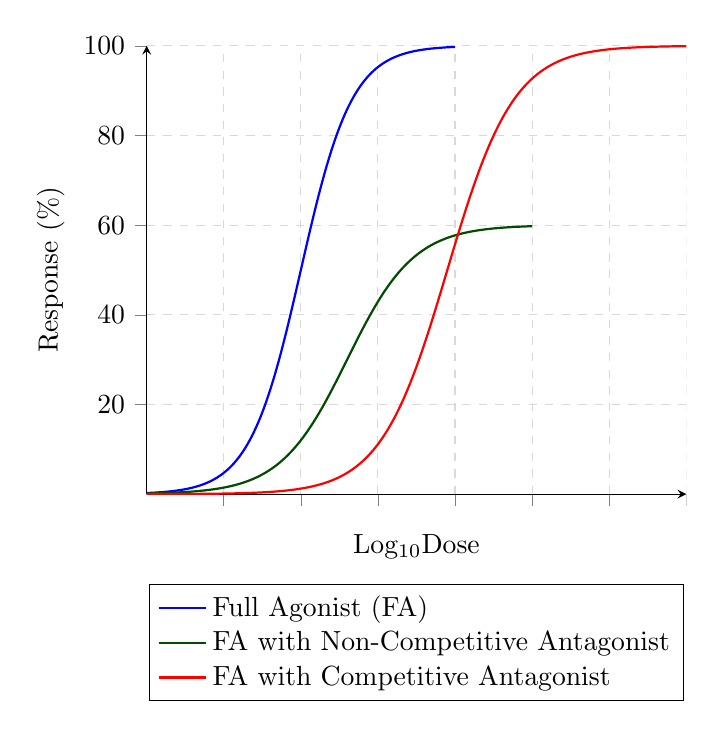
\begin{tikzpicture}
    \begin{axis}[
        axis x line=middle,
        axis y line=middle,
        x tick label style={/pgf/number format/fixed,
                            /pgf/number format/fixed zerofill,
                            /pgf/number format/precision=1},
        y tick label style={/pgf/number format/fixed,
                            /pgf/number format/fixed zerofill,
                            /pgf/number format/precision=0},
        grid = major,
        grid style={dashed, gray!30},
        xmin=0,     % start the diagram at this x-coordinate
        xmax= 0.7,    % end   the diagram at this x-coordinate
        ymin= 0,     % start the diagram at this y-coordinate
        ymax= 100,   % end   the diagram at this y-coordinate
        %axis background/.style={fill=white},
    	  x label style={at={(axis description cs:0.5,-0.1)},anchor=north},
	  y label style={at={(axis description cs:-0.1,.5)},rotate=90,anchor=south},
	  xticklabels={},
	 ylabel near ticks,
	xlabel near ticks,
        xlabel=Log\textsubscript{10}Dose,
        ylabel=Response (\%),
        tick align=outside,
        enlargelimits=false,
legend style={at={(0.5,-0.2)},anchor=north},
legend cell align={left}
]
	\coordinate (o) at (0,0);
     \addplot[domain=0:0.4, blue, thick,samples=500] {100*(1/(1+exp(-30*(x-0.2))))};
\addlegendentry{Full Agonist (FA)};
	\addplot[domain=0:0.5, green!30!black, thick,samples=500] {60*(1/(1+exp(-30*((x/1.3)-0.2))))};
\addlegendentry{FA with Non-Competitive Antagonist};
	\addplot[domain=0.0:0.7, red, thick,samples=500] {100*(1/(1+exp(-30*((x/1.3)-0.3))))};
\addlegendentry{FA with Competitive Antagonist}; 

\end{axis}

\end{tikzpicture} 
\end{document}

